We propose an alternative method based on spectral clustering for obtaining local labor market definitions. We refer to definitions based on this methodology as Mobility Zones, but note that the methodology is still under development and that mappings presented here are preliminary. We first describe spectral clustering, then show the results of our implementation, and then compare our definitions with Tolbert and Sizer's commuting zones and other local labor market defintions using our objective function.

%Our initial technique uses a disjoint cluster analysis, usually called a k-means model. The k-means clustering algorithm works in the following way. Consider a set of $N$ observations, with $k$ variables that are associated with them. For example, a county can have a latitude, longitude, and unemployment rate. This vector of variables for observation $i$ is $X_i$. The distance between $X_i$ and $X_j$ is defined by a function $d(X_i,X_j)$, which is normally the Euclidian distance between the observations.\footnote{In order to ensure that scales are the same, all components of $X_i$ are normalized before calculating the distance.} Given a number of clusters $M$, the k-means algorithm selects (or is given) a set of starting cluster centers, ${m_1,\dots,m_M}$. Given this initial set of seeds, each observation $i$ is assigned to a cluster $c$ if
%\[
%d(X_i,m_c) << d(X_i,m_d) \, \, \, \forall d \neq c
%\]
%After all observations are assigned to a cluster, the new cluster seeds are assigned as the means of clusters, such that the new center for cluster $c$ is $m_c =\bar{X}_c$.
%This process is then iterated until convergence, so that $d(m_c,\bar{X}_c) < \epsilon$ for some specified $\epsilon$. 

%Since we do not want to impose a number of clusters  \emph{a priori}, we iterate over a number of different values for $M$, the maximum number of clusters. Additionally, one known issue with k-means clustering procedures is that the output is sensitive to starting values. For this reason, for each value of $M$, we iterate the procedure with a number of different starting seeds.\footnote{To get these starting seeds, we randomly choose M counties without replacement. In future work we are going to test the sensitivity of other sampling methods.} For each combination of seeds $s$ and number of clusters $M$, we calculate the objective function, and choose the definition with the lowest value for the objective function.

%In our first pass at using this method, we only include population centroid latitude and longitude, which ensures that the labor market clusters that we get are similar in size geographically. Additionally, we use 1990 data in the objective function in selecting the optimal cluster set. This method yields the clusters in Figure \ref{fig:fastclusmap}.

%\begin{figure}[th]
\caption{Outcome of K-Means Clustering}
%\begin{subfigure}[t]{0.5\textwidth}
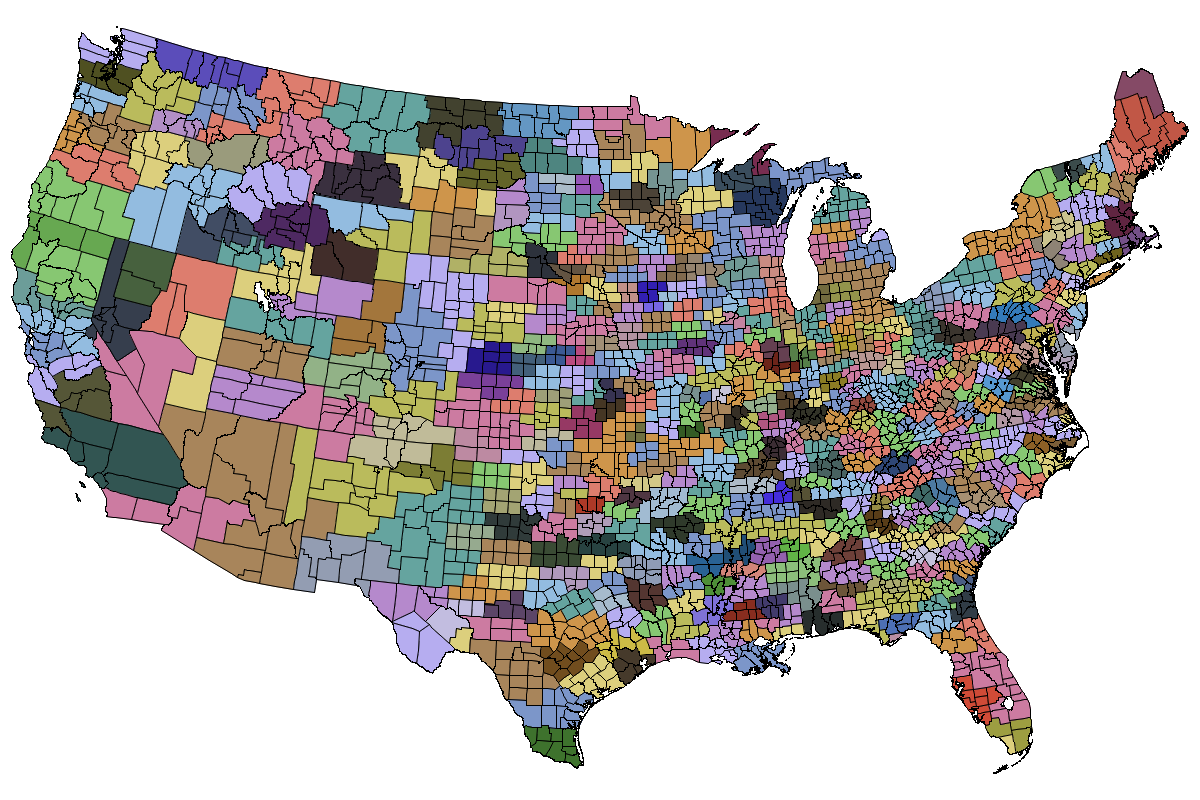
\includegraphics[width=.9\textwidth]{./figures/fastclus_map.png}
\label{fig:fastclusmap}
\end{figure}


%We graph the objective function value of this labor market definition in Figure \ref{fig:objfn_norm_fastclus}, labelled ``fastclus," comparing it with the other local labor market definitions. We find that while this definition initially does better than state, it is still less appropriate than 1990 and 2000 Commuting Zones. The likely cause is that our candidate areas are only selected based on geographic proximity; our next step is to include economic variables  such as wages and unemployment rates in the clustering method, which will \mc{likely improve our outcomes.}{ADF: Do we want a map of our resulting zones? Or will that not help? Or some quick summary statistics?} In theory, by minimizing the objective function, we should be able to arrive at a definition of labor markets that is at least as good as the Commuting Zone definition. Our ability to improve on the definitions will depend on developing improved methods for proposing candidate mappings of counties to clusters.

%\subsection{Spectral Clustering}



\subsection{Introduction to Spectral Clustering}

Spectral clustering classifies nodes by implementing k-means on the eigenvectors of a graph Laplacian of pairwise similarities \citep{vonLuxburg2007}. Spectral clustering can be explained as a random walk on the similarity graph, where the probability of jumping from one node to another is given by edge weights. In the stationary distribution of these stochastic jumps, a clustering may be thought of as the classification that minimizes jumps between clusters, for a given number of clusters. This interpretive framework is a natural way to think of local labor markets and job search or migration models. For this work, we assume an undirected or symmetric graph of similarities. Spectral clustering is a popular methodology implemented in a wide range of fields.

We implement normalized spectral clustering as defined by \cite{NgJordanWeiss2001}, which re-normalizes the rows of the eigenvectors for the number of clusters specified. This re-normalization has the advantage that even fairly isolated nodes end up clustered. In our experience, both hierarchical clustering and standard versions of spectral clustering were highly sensitive to the intensity of commuting flows and often failed to differentiate clusters outside of major urban centers. These residual, mostly rural, areas would end up lumped into a ``mega-cluster'' with little geographic integrity. Only by saturating the model with a high number of clusters (or a high threshold in the case of hierarchical clustering) could we allocate all counties to similarly sized clusters. With the methodology of \cite{NgJordanWeiss2001}, we can reliably allocate all counties to clusters for any quantity of clusters that we specify. We rely on the objective function to determine the optimal quantity of clusters, as implemented by normalized spectral clustering.

Spectral clustering is also amenable to classifying nodes based on multiple views of a graph, as we have argued is appropriate for characterizing local labor markets. Nodes may be characterized both by the intensity of pairwise links (.e.g commuting flows, distance, correlation of unemployment rates) and by feature space similarity (e.g. share employed in manufacturing). \cite{ZhouBurges2007} generalize single-view spectral clustering, showing that multi-views can be summarized in an undirected similarity graph as a weighted, linear combination of each view. Considering again the random walk interpretation of spectral clustering, \cite{ZhouBurges2007} interpret the multi-view graph as a mixture of Markov transition chains for each view. The objective function, which is also a linear combination of weighted values for each cluster, is not necessarily helpful for selecting an optimal weights. In the current implementation, we assign an equal linear weight to each view in the multi-view graph, using the same views that enter into the objective function. As with the objective function, the linear weights would depend on the economic interpretation of the clusters. 

The following, using notation from \cite{vonLuxburg2007}, describes the specific steps of our implementation of multi-view spectral clustering, with the goal of classifying $n$ counties into $k$ clusters:
\begin{enumerate}
   \item We construct an undirected similarity graph $S$, where the edge weights between nodes $i$ and $j$ are defined as $w_{ij}$, with the weight consisting of a linear combination of the set of views (e.g. commute flows, proximity, pairwise corrleation in unemployment rates).
   \item We compute the Laplacian, a symmetric matrix, as $L=Deg(S)^{-1/2}\cdot S \cdot Deg(S)^{-1/2}$, where $Deg(S)$ is the Degree matrix giving the row sums of $S$ on the diagonal.
   \item We compute eigenvalues and eigenvectors of $L$ and form an $n$ by $k$ matrix, $U$, from the $k$ eigenvectors with the largest eigenvalue.
   \item We form an $n$ by $k$ matrix $T$ by normalize the rows of $U$ to norm 1, each element $t_{ij}=u_{ij}/(\sum_{j \in k}u_{ik}^{2})^{1/2}$.
   \item We classify the $n$ rows of $T$ (one for each county) into $k$ clusters, $C_{1}, ... ,C_{k}$ using the k-means algorithm.
\end{enumerate}

\subsection{Implementation of Spectral Clustering}

In implementing this methodology, we use the similarity matrix implied by TS1996 as $S$, over which the Laplacian is computed. Additionally, in spectral clustering, the choice variable is not the cutoff height (as in hierarchical clustering) but the number of clusters, $k$. Rather than arbitrarily choose a number of clusters, we use our objective function specificed in equation \ref{eqn:objfn} to choose the set of clusters that is the most integrated, such that $k$ maximizes our objective function. Formally, we choose k such that:


\[
k*: ObjFn(C_{k*}) = \max\limits_{k \in [400,800]} ObjFn (C_k)
\]

Our resulting clusters are mapped in Figure \ref{fig:spectral}, and our calculations show that the optimal number of clusters is 656. Additionally, using our methodoogy clusters have an average of 4.74 counties each, which is larger than Tolbert and Sizer's defintions (4.24). Comparing Figure \ref{fig:spectral} with Tolbert and Sizer's commuting zones, there are a number of differences. First, our clusters are somewhat larger geographically. Second, the clusters in the East are larger in area than the clusters in Tolbert and Sizer's definitions. This is particularly telling in Florida, which has fewer clusters using our definitions. The same is true of Texas; in our clusters, the main metropolitan areas are visible, while they are not in Tolbert and Sizer. One notable similarity are the high frequency of very small clusters in Kansas. It appears that irrespective of methodology, there is not a lot of long-distance commuting in Kansas, which may reflect the different industrial composition.

\begin{figure}
\caption{Optimal Spectral Output, 656 Clusters\label{fig:spectral}}
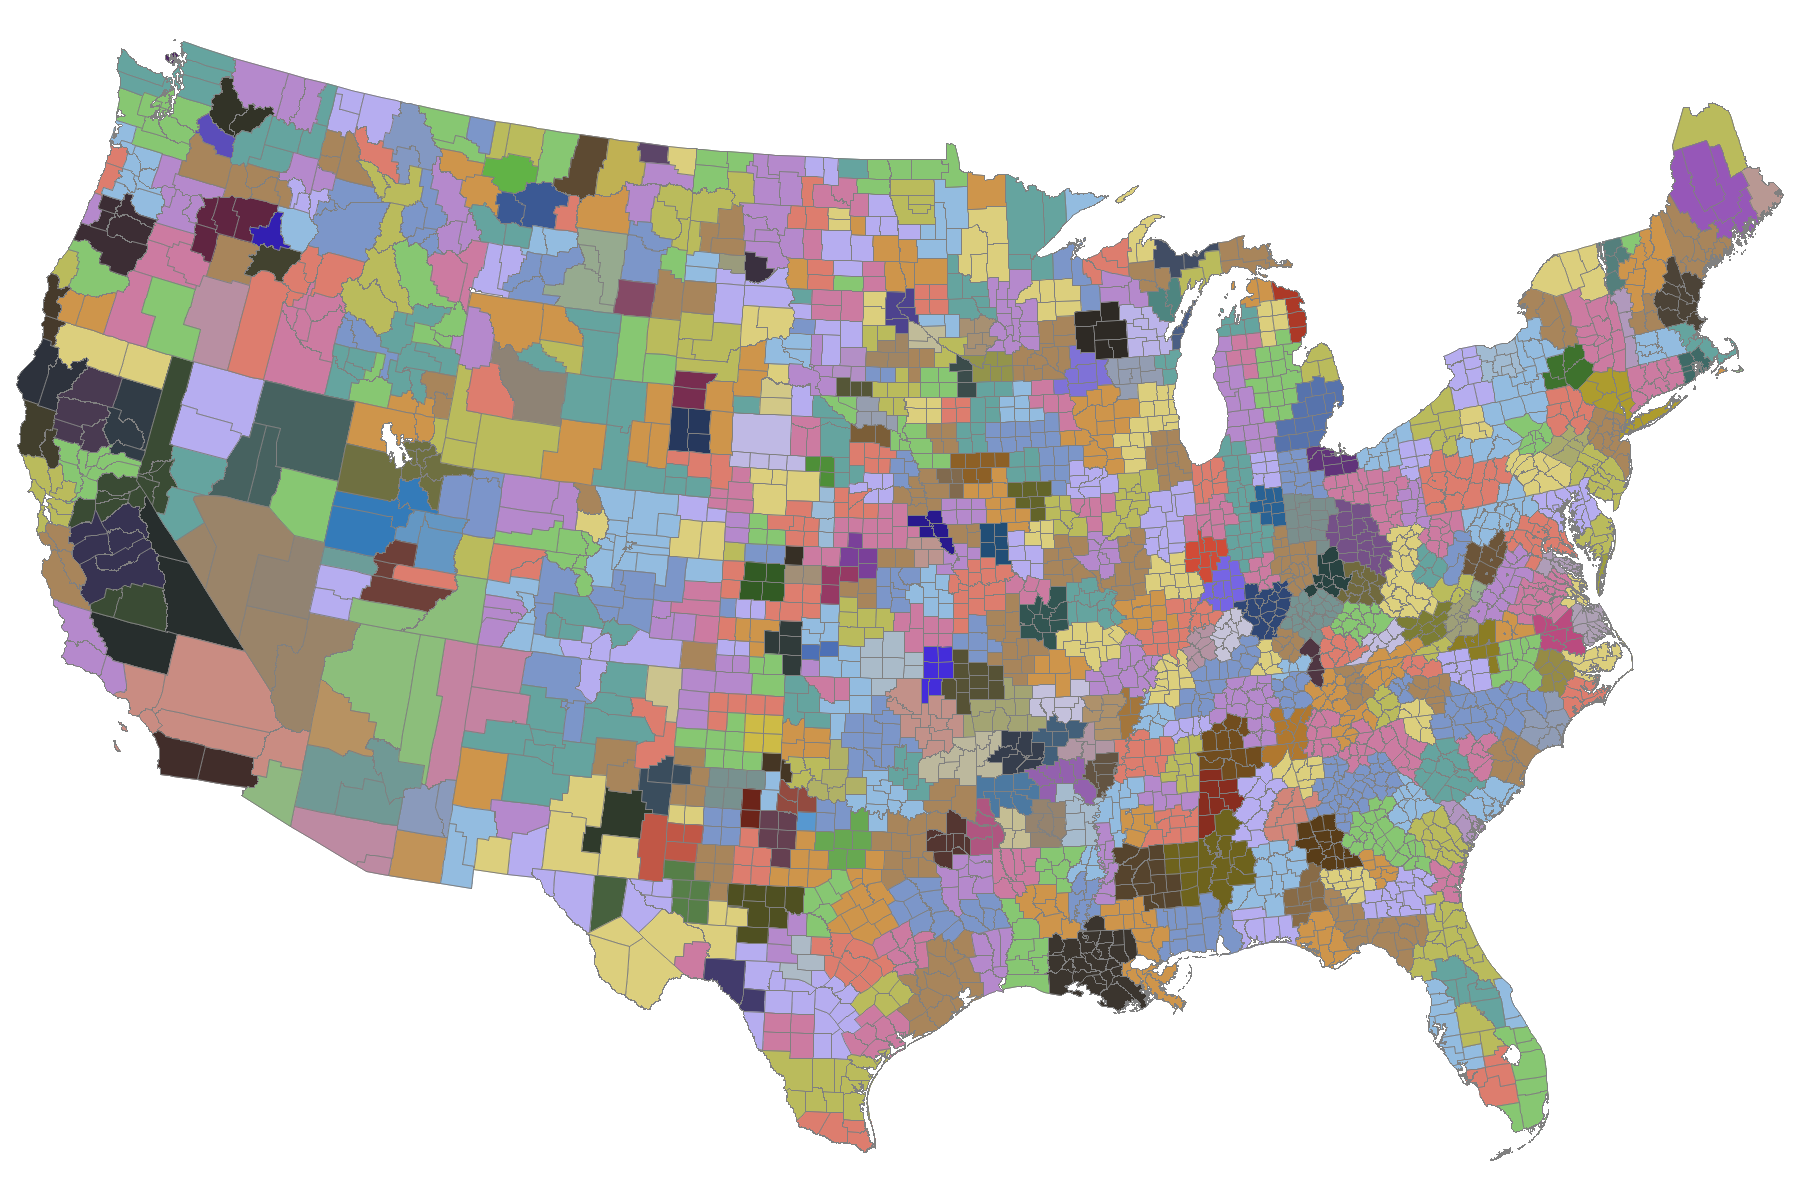
\includegraphics[scale=.4]{./figures/optimal_spectral_par.png}
\footnotesize \emph{Note:} Clusters are a result of authors' calculations, using methodology outlined in text.
\end{figure}

Next, we turn to comparing our results from the spectral clustering method with other local labor market definitions, using our objective function.

\subsection{Comparing Common Local Labor Market Definitions}

To compare our definitions to other candidate local labor markets, we calculate the objective function for a number of candidate local labor markets: our maximized spectral clustering definintion, Tolbert and Sizer's commuting zones, states, CBSAs (with a non-metro state residual), CBSAs only, and counties. These results are displayed in Figure \ref{fig:objfn_results}.

\begin{figure}\centering
\caption{Comparing Different Local Labor Market Definitions}
\begin{tabular}{c}
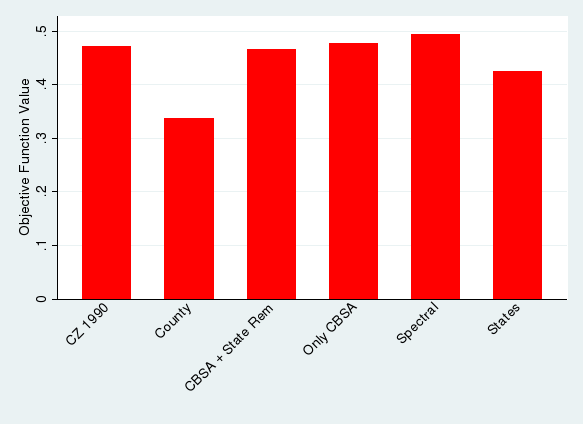
\includegraphics[scale=0.45]{./figures/objectivefunction_defns.png}\\
\multicolumn{1}{p{4.5in}}{\footnotesize \emph{Notes:} Author's calculations. CBSA definitions are 2010 current definitions. Data used in these calculations are discussed in Section \ref{sec:data}.}
\end{tabular}
\label{fig:objfn_results}
\end{figure}

Spectral clustering outperforms all other labor market definitions, while commuting zones are the next best option. If we use CBSAs and rest of state, our analysis shows that is somewhat on par with commuting zone definitions, while CBSA-only definitions only slightly outperform CBSA and state residuals. Finally, our analysis appears to suggest that counties are a poor representation of a local labor market compared with any other definition, even states.

In future work, we also want to compare these definitions over time, to see whether the decay in quality of local labor market definition is different across these definitions. This is especially relevant for current research which uses commuting zones, since these areas may not reflect current local labor market definitions.
